When we apply the \sts model to response generation, one severe issue stands out:
neural conversation models tend to generate 
dull responses such
 \textit{I~don't know} or  \textit{I ~don't know what you are talking about} \cite{serban2015hierarchical,vinyals2015neural}. 
From Table \ref{sample:mle}, we can see that
many top-ranked responses are generic. %, along the lines of  \textit{I don't know} or \textit{Oh my god!}
Responses that seem more meaningful or specific can also be found in the N-best lists, but rank much lower.
This phenomenon is due to the 
 relatively high frequency of generic responses like 
 \textit{I don't know} in conversational datasets.
 The MLE (maximum likelihood estimation) objective function models the uni-directional dependency from sources to targets, 
 and since 
 dull responses are dull in the similar way and diverse responses are diverse in different ways, the system always generates these dull responses. 
 Intuitively, it seems desirable to take into account not only the dependency of responses on messages, but also the inverse, the likelihood that a message will be provided to a given response:
 it is hard to guess what an input message is about knowing that the response is {\it i don't know}.
 
\begin{table}[!ht]
\center
\small
\begin{tabular}{ll}\toprule
\multicolumn{2}{l}{{\bf Input}: What are you doing?}  \\\midrule
-0.86~~I don't know.&-1.09~~Get out of here.\\
-1.03~~I don't know!&-1.09~~I'm going home. \\
-1.06~~Nothing.& -1.09~~Oh my god! \\
-1.09~~Get out of the way.&-1.10~~I'm talking to you.\\\midrule
\multicolumn{2}{l}{{\bf Input}: what is your name?} \\\midrule 
-0.91~~I don't know. & ... \\
-0.92~~I don't know! & -1.55~~My name is Robert.\\
-0.92~~I don't know, sir.&-1.58~~My name is John. \\
-0.97~~Oh, my god!& -1.59~~My name's John. \\\midrule
\multicolumn{2}{l}{{\bf Input}: How old are you?} \\\midrule 
-0.79~~I don't know. & ... \\
-1.06~~I'm fine.& -1.64~~Twenty-five. \\
-1.17~~I'm all right. & -1.66~~Five.\\
-1.17~~I'm not sure. & -1.71~~Eight. \\\bottomrule
\end{tabular}
\caption[Sample responses  from vanilla \sts neural models]{Responses generated by a 4-layer \sts neural model trained on 20 million conversation pairs take from the OpenSubtitles dataset.
Decoding is implemented with beam size set to 200. The top examples are the responses with the highest average probability log-likelihoods in the N-best list. Lower-ranked, less-generic responses were manually chosen.} 
\label{sample:mle}
\end{table}


We propose to capture this intuition by using Maximum Mutual Information (MMI), as an optimization objective that measures the mutual dependence between inputs and outputs, as opposed to 
the uni-directional dependency from sources to targets in the traditional MLE objective function.
We present practical training and decoding strategies for neural generation models that use MMI as objective function.
We demonstrate that using MMI results in a clear decrease in the proportion of generic response sequences, and 
find a significant performance boost from the proposed models as measured by  BLEU \cite{papineni2002bleu} and human evaluation.


\section{MMI Models}
In the response generation task,
let $x$ denote an input message sequence (source) $x=\{x_1,x_2,...,x_{n_x}\}$ where $n_x$ denotes the number of words in $x$.
Let $y$ (target) denote a sequence in response to source sequence $x$, where $y=\{y_1,y_2,...,y_{n_y},$ \eos{}\}, $n_y$ is the length of the response (terminated by an \eos token). $V$ denotes vocabulary size. 

\subsection{MMI Criterion}
The standard objective function for sequence-to-sequence models is the log-likelihood of target $y$ given source $x$, which at test time yields the statistical decision problem:
\begin{equation}
\hat{y}= \argmax_y \big\{\log p(y|x)\big\}
\label{eqseq2seq}
\end{equation}
As discussed in the introduction, we surmise that this formulation leads to generic responses being generated, since it only selects for targets given sources, not the converse. 
To remedy this, we replace it with Maximum Mutual Information (MMI) as the objective function. 
In MMI, parameters are chosen to maximize (pairwise) mutual information
between the source $x$ and the target $y$:
\begin{equation}
\log \frac{p(x,y)}{p(x)p(y)}
\label{eq1}
\end{equation}

This avoids favoring responses that unconditionally enjoy high probability, and instead biases towards those responses that are specific to the given input.
The MMI objective can be written as follows:\footnote{Note: $\log\frac{p(x,y)}{p(x)p(y)} = \log\frac{p(y|x)}{p(y)} = \log p(y|x) - \log p(y)$}
\begin{equation*}
\begin{aligned}
\hat{y} = \argmax_{y} \big\{\log p(y|x) - \log p(y)\big\}
\end{aligned}
\end{equation*}
%
We use a generalization of the MMI objective which introduces a hyperparameter $\lambda$ that controls how much to penalize generic responses:
\begin{equation}
\hat{y}  =\argmax_{y} \big\{\log p(y|x) - \lambda\log p(y)\big\}
\label{eqweightedmmi}
\end{equation}

An alternate formulation of the MMI objective uses Bayes' theorem:
\begin{equation*}
\log p(y)=\log p(y|x)+\log p(x)-\log p(x|y)
\label{eqbayes}
\end{equation*}
which lets us rewrite Equation \ref{eqweightedmmi} as follows:
\begin{equation}
\begin{aligned}
\hat{y}%&=\argmax_{T} \big\{\log p(T|S)-\lambda\log p(T)\big\}\\
&=\argmax_{y} \big\{(1-\lambda)\log p(y|x)\\
&~~~~~~~~~~~~~~~~+\lambda\log p(x|y)-\lambda\log p(x) \big\} \\[0.2cm]
&=\argmax_{y} \big\{(1-\lambda)\log p(y|x)+\lambda\log p(x|y) \big\}
\label{eqbayesexpanded}
\end{aligned}
\end{equation}
This weighted MMI objective function can thus be viewed as representing a tradeoff between sources given targets (i.e., $p(x|y)$) and targets given sources (i.e., $p(y|x)$). 

We would like to be able to 
adjust the value $\lambda$ in Equation \ref{eqweightedmmi} without repeatedly training neural network models from scratch, which would otherwise be extremely time-consuming.
Accordingly, we did not train a joint model ($\log p(y|x) - \lambda \log p(y)$), but instead trained maximum likelihood models, and used the MMI criterion only during testing.

\subsection{Practical Considerations}
Responses can be generated either from Equation~\ref{eqweightedmmi},  i.e., $\log p(y|x)-\lambda \log p(y)$ or Equation~\ref{eqbayesexpanded}, i.e., $(1-\lambda) \log p(y|x)+\lambda \log p(x|y)$. 
We will refer to these formulations as \mmiLM and \mmiBD, respectively.
However, these strategies are difficult to apply directly to decoding since they can lead to ungrammatical responses 
(with \mmiLM)
or make decoding intractable 
(with \mmiBD).
In the rest of this section, we will discuss these issues and explain how we resolve them in practice. 
 
\subsubsection{\mmiLM}
The second term of $\log p(y|x)-\lambda \log p(y)$
functions as an anti-language model.
It penalizes not only high-frequency, generic responses, but also fluent ones and thus can lead to ungrammatical outputs. 
In theory, this issue should not arise when $\lambda$ is less than~1, since ungrammatical sentences should always be more severely penalized by the first term of the equation, i.e., $\log p(y|x)$.
 In practice, however, we found that the model tends to select ungrammatical outputs that escaped being penalized by $p(y|x)$. 
 
\paragraph{Solution}
Let $n_y$ be the length of target $y$.
$p(y)$ in Equation~\ref{eqweightedmmi} can be written as:
\begin{equation}
p(y)=\prod_{i=1}^{n_y}p(y_i|y_1,y_2,...,y_{i-1})
\end{equation}
We replace the language model $p(y)$ with $U(y)$, which adapts the standard language model by multiplying by a weight $g(i)$ that is decremented monotonically as the index of the current token $i$ increases:
\begin{equation}
\begin{aligned}
U(y)=\prod_{i=1}^{n_y}p(t_i|t_1,t_2,...,t_{i-1})\cdot g(i)
\end{aligned}
\label{eqmonotonic}
\end{equation}
The underlying intuition here is as follows:
First, neural decoding combines the previously built representation with the word predicted at the current step. 
As decoding proceeds, the influence of the initial input on decoding (i.e., the source sentence representation) diminishes as additional previously-predicted words are encoded in the vector representations.\footnote{Attention models \cite{xu2015show} may offer some promise of addressing this issue.}
In other words, the first words to be predicted significantly determine the remainder of the sentence. 
Penalizing words predicted early on by the language model contributes more to the diversity of the sentence than it does to words predicted later. 
Second, as the influence of the input on decoding declines, 
the influence of the language model comes to dominate. 
We have observed that ungrammatical segments tend to appear in the latter part of the sentences, especially in long sentences. 

We adopt the most straightforward form of $g(i)$ by 
by setting up a threshold ($\gamma$) by penalizing the first $\gamma$ words where\footnote{We experimented with a smooth decay in $g(i)$ rather than a stepwise function, but this did not yield better performance.}
\begin{equation}
\begin{aligned}
g(i)
= \left\{
\begin{aligned}
&1~~~~~\text{if}~i\leq\gamma \\
&0~~~~~\text{if}~i>\gamma
\end{aligned}
\right.
\end{aligned}
\end{equation}
The objective Equation \ref{eqweightedmmi} 
can thus be rewritten as: 
\begin{equation}
\begin{aligned}
\log p(y|x) - \lambda \log U(y)
\end{aligned}
\label{eqweightedpos}
\end{equation}
where direct decoding is tractable.
 
\subsubsection{\mmiBD}
Direct decoding from \mmiBDv is intractable, as the second part (i.e., $p(s|t)$) requires completion of 
target generation \textit{before} $p(s|t)$ can be effectively computed.
Due to the enormous search space for target $y$, exploring all possibilities is infeasible. 

For practical reasons, then, we turn to an approximation approach that involves first generating \mbox{N-best} lists given the first part of objective function, i.e., 
standard \sts model $p(t|s)$. 
Then we rerank the \mbox{N-best} lists using the second term of the objective function. 
Since N-best lists produced by \sts models are generally grammatical, the final selected options are likely to be well-formed. 
Model reranking has obvious drawbacks. It results in non-globally-optimal solutions by first emphasizing standard \sts objectives. 
Moreover, it relies heavily on the system's success in generating a sufficiently diverse N-best set, requiring that a long list of N-best lists be generated for each message. 
This assumption is far from valid as one long-recognized issue with beam search is
lack of diversity in the beam: candidates often differ
only by punctuation or minor morphological variations,
with most of the words overlapping. 
The lack
of diversity in the N-best list significantly decreases
the impact of reranking. This means we need a more diverse N-best list for the later re-ranking process. 
\paragraph{Standard Beam-search Decoding}
Here, we first give a sketch of the standard beam-search model and then talk about how we can modify it to produce more diverse N-best lists. 
In standard beam-search decoding, 
 at time step $t-1$ in decoding, the decoder keeps track of $K$ hypotheses, where $K$ denotes the beam size, and their scores $S(y_{1:t-1}|x)=\log p(y_1,y_2,...,y_{t-1}|x)$. As it moves on to time step $t$,
it expands each of the $K$ hypotheses
(denoted as $y_{1:t-1}^k=\{y_1^k,y_2^k,...,y_{t-1}^k\}$, $k\in [1,K]$)
 by selecting the top $K$ candidate expansions,  each expansion
 denoted as  $y_t^{k,k'}$, $k'\in [1,K]$,
  leading to the construction of $K\times K$ new hypotheses:
  $$[Y_{t-1}^k, y_t^{k,k'}], k\in [1,K], k'\in [1,K]$$
The score for each of the $K\times K$ hypotheses is computed as follows:
\begin{equation}
S(y_{1:t-1}^k,y_t^{k,k'}|x)=S(y_{1:t-1},x)+\log p(y_t^{k,k'}|x,y_{1:t-1}^k)
\end{equation}
In a standard beam search model, the top $K$ 
hypotheses are selected
(from the $K\times K$  hypotheses computed in the last step) based on 
the score $S(y_{1:t-1}^k,y_t^{k,k'}|x)$. The remaining hypotheses are ignored when the algorithm proceeds to the next time step.
\begin{figure*}
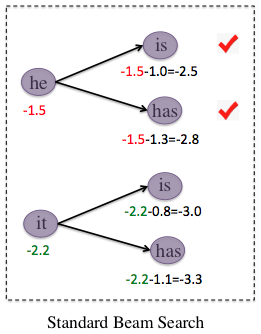
\includegraphics[width=2in]{img/diverse1.png}
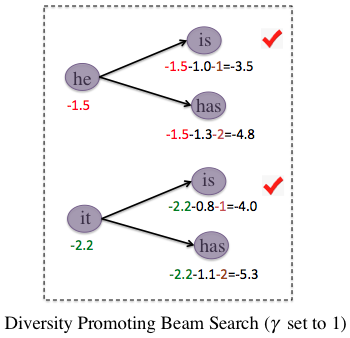
\includegraphics[width=2.6in]{img/diverse2.png}
\centering
\caption[Standard beam search vs the diversity-promoting beam search]{An illustration of standard beam search and the proposed diversity-promoting beam search. $\gamma$ denotes the hyperparameter for penalizing intra-sibling ranking. Scores are made up for illustration purposes. }
\label{figure}
\end{figure*}




\paragraph{Diversity-Promoting Beam Seach}
We propose to increase diversity by changing
the way $S(Y_{t-1}^k,y_t^{k,k'}|x)$ is computed,
as shown in Figure \ref{figure}.
For each of the  hypotheses $Y_{t-1}^k$ ({\it he} and {\it it}),
we generate the top $K$ translations
 $y_t^{k,k'}$, $k'\in [1,K]$ as in the standard beam search model.
Next, we  rank the $K$ translated tokens generated from the same parental hypothesis
based on $p(y_t^{k,k'}|x,Y_{t-1}^k)$ 
in descending order: {\it he is} ranks first among {\it he is} and {\it he has}, and {\it he has} ranks second;
similarly for {\it it is} and {\it it has}.
 
We then rewrite the score for $[Y_{t-1}^k, y_t^{k,k'}]$ by adding an additional term $\gamma k'$,
 where $k'$ denotes the ranking of the current hypothesis among its siblings (1 for {\it he is} and {\it it is}, 2 for {\it he has} and {\it it has}).
\begin{equation}
\hat{S}(Y_{t-1}^k,y_t^{k,k'}|x)=S(Y_{t-1}^k,y_t^{k,k'}|x)-\gamma k'
\label{dive}
\end{equation}
We call $\gamma$ the {\it diversity rate}; it indicates the degree of diversity one wants to integrate into the beam search model.

The top $K$ hypotheses are selected based on $\hat{S}(Y_{t-1}^k,y_t^{k,k'}|x)$ as we move on to the next time step.
By adding the additional term $\gamma k'$, 
the model punishes lower-ranked hypotheses among siblings (hypotheses descended from the same parent).
When we compare newly generated hypotheses descended from different ancestors, the model gives more credit to  top hypotheses from each of the different ancestors.
For instance, even though the original score for {\it it is} is lower than {\it he has},
the model favors the former as the latter is more severely punished by the intra-sibling ranking part $\gamma k'$. 
The model thus generally favors choosing hypotheses from diverse parents, leading to a more diverse N-best list. 
The proposed model is straightforwardly implemented with a minor adjustment to the standard beam search.

\subsection{Training}

Recent research has shown that deep LSTMs work better than single-layer LSTMs for \sts tasks \cite{sutskever2014sequence}.
We adopt a deep structure with four LSTM layers for encoding and four LSTM layers for decoding, each of which consists of a different set of parameters. 
Each LSTM layer consists of 1,000 hidden neurons, and the dimensionality of word embeddings is set to 1,000. 
Other training details are given below, broadly aligned with \newcite{sutskever2014sequence}. 
\begin{itemize}[noitemsep,nolistsep]
\item LSTM parameters and embeddings are initialized from a uniform distribution in [-0.08, 0.08].
\item Stochastic gradient decent is implemented using a fixed learning rate of 0.1. 
\item Batch size is set to 256.
\item Gradient clipping is adopted by  scaling gradients when the norm exceeded a threshold of 1. 
\end{itemize}
Our implementation on a single GPU processes at a speed of approximately 600-1200 tokens per second.\footnote{Tesla K40m, 1 Kepler GK110B, 2880 CUDA cores.} 

The $p(y|x)$ model described in Section 4.3.1 was trained using the same model as that of $p(y|x)$, with messages ($x$) and responses ($y$) interchanged.

\subsection{Decoding}
\subsubsection{\mmiLM}
As described in Section 4.3.1, decoding using \mmiLMv %this model
 can be readily implemented by predicting tokens at each time-step.
 In addition, we found in our experiments that it is also important to take into account the length of responses in decoding.
 We thus linearly combine the loss function with length penalization, leading to an ultimate score for a given target $T$ as follows:
 \begin{equation}
 Score(T)=p(y|x)-\lambda U(y)+\gamma L_y
 \end{equation}
where $L_T$ denotes the length of the target and $\gamma$ denotes associated weight. We optimize $\gamma$ and $\lambda$ using MERT \cite{och2003minimum} on N-best lists of response candidates. 
The N-best lists  are generated using the decoder with beam size 200.
We set a maximum length of 20 for generated candidates. 
At each time
step of decoding, we are presented with $N\times N$
word candidates. We first add all hypotheses with
an EOS token being generated at current time step
to the N-best list. Next we preserve the top N
unfinished hypotheses and move to next time step.
We therefore maintain batch size of 200 constant
when some hypotheses are completed and taken
down by adding in more unfinished hypotheses.
This will lead the size of final N-best list for each
input much larger than the beam size.



\subsubsection{\mmiBD}
We  generate N-best lists based on $P(T|S)$ and then rerank the list by linearly combining $p(T|S)$, $\lambda p(S|T)$, and $\gamma L_T$. We use MERT \cite{och2003minimum} to tune the 
weights $\lambda$ and $\gamma$ on the development set. 



\begin{table*}
\center
\small
\begin{tabular}{lcccc}\toprule
%Model                                &$\#$ of Training Data ($\approx$) &\bleu       &{\it distinct-1}      &{\it distinct-2}\\\hline
Model                                  &$\#$ of training instances        &\bleu         &{\it distinct-1}      &{\it distinct-2}\\
\sts (baseline)                        & 23M                              & 4.31         & .023               & .107\\
\sts (greedy)                          & 23M                              & 4.51         & .032               & .148\\
\multirow{1}{*}{\mmiLM: \mmiLMv}& \multirow{1}{*}{23M}          &  4.86   & .033              & .175\\
%                                      &                                  & (+x.x$\%$)   & (+xx.x$\%$)        & (+xx.x$\%$)\\\hline
\multirow{1}{*}{\mmiBD: \mmiBDv}&\multirow{1}{*}{23M}& {\bf 5.22} & .051               & .270\\ 
%                                      &                                  & (+xx.x$\%$)  & (+xx.x$\%$)        & (+xx.x$\%$)\\\hline\hline
SMT \cite{ritter2011data}              & 50M                              & 3.60         & .098               & .351\\
SMT+neural reranking \cite{sordoni2015neural}& 50M                              & 4.44         & {\bf .101}         & {\bf .358}\\\bottomrule
\end{tabular}
\caption[Performance on the Twitter dataset of \sts models and MMI models]{Performance on the Twitter dataset of 4-layer \sts models and MMI models. {\it distinct-1} and {\it distinct-2} are respectively the number of distinct unigrams and bigrams divided by total number of generated words.}
\label{res:twitter}
\end{table*}
\section{Experiments}
\subsection{Datasets}
\paragraph{Twitter Conversation Triple Dataset} 
We used an extension of the dataset described in 
\newcite{sordoni2015neural}, which consists of 23 million conversational snippets randomly selected from a collection of 129M context-message-response triples extracted from the Twitter Firehose over the 3-month period from June through August 2012.
For the purposes of our experiments, we limited context to the turn in the conversation immediately preceding the message. In our LSTM models, we used a simple input model in which contexts and messages are concatenated to form the source input. 

For tuning and evaluation, we used the development dataset (2118 conversations) and the test dataset (2114 examples), augmented using information retrieval methods to create a multi-reference set. 
The selection criteria for these two datasets included a component of relevance/interestingness, with the result that dull responses will tend to be penalized in evaluation.

\paragraph{OpenSubtitles Dataset} In addition to unscripted Twitter conversations, we also used the OpenSubtitles (OSDb) dataset \cite{tiedemann2009news}, a large, noisy, open-domain dataset containing roughly 60M-70M scripted lines spoken by movie characters. 
This dataset does not specify which character speaks each subtitle line, which prevents us from inferring speaker turns. 
Following Vinyals et al. (2015), we make the simplifying assumption that each line of subtitle constitutes a full speaker turn. Our models are trained to predict the current turn given the preceding ones based on the assumption that consecutive turns belong to the same conversation.
This introduces a degree of noise, since consecutive lines may not appear in the same conversation or scene, and may not even be spoken by the same character.

This limitation potentially renders the OSDb dataset unreliable for evaluation purposes.  
For evaluation purposes, we therefore used data from the Internet Movie Script Database (IMSDB),\footnote{IMSDB (\url{http://www.imsdb.com/}) is a relatively small database of around 0.4 million sentences and thus not suitable for open domain dialogue training.} which explicitly identifies which character speaks each line of the script. 
This allowed us to identify consecutive message-response pairs spoken by different characters. %within the same scene. 
We randomly selected two subsets as development and test datasets, each containing 2K pairs, with source and target length restricted to the range of [6,18]. 

\begin{table}
\center
\small
\begin{tabular}{cccc}\toprule
Model&\bleu&{\it distinct-1}&{\it distinct-2}\\\midrule
\sts&7.16&0.0420&0.133\\
\mmiLM&7.60 & 0.0674&0.220\\
\mmiBD&8.26&0.0758&0.288\\\bottomrule
\end{tabular}
\caption[Performance on the OpenSubtitles dataset for MMI models]{Performance on the OpenSubtitles dataset for the \sts baseline and two MMI models.}
\label{res:open}
\end{table}

\subsection{Evaluation}
For parameter tuning and final evaluation,
we used \bleu \cite{papineni2002bleu}, which was shown to correlate reasonably well with human judgment on the response generation task \cite{galley2015deltableu}.
In the case of the Twitter models, we used multi-reference \bleu. 
As the IMSDB data is too limited to support extraction of multiple references, only single reference \bleu was used in training and evaluating the OSDb models.

We did not follow  \newcite{vinyals2015neural} in using perplexity as evaluation metric. 
Perplexity is unlikely to be a useful metric in our scenario, since our proposed model is designed to steer away from the standard \sts model in order to diversify the outputs.   
We report degree of diversity by calculating the number of distinct unigrams and bigrams in generated responses. The value is scaled by total number of generated tokens to avoid favoring long sentences (shown as {\it distinct-1} and {\it distinct-2} in Tables \ref{res:twitter} and \ref{res:open}). 

\subsection{Results}

\paragraph{Twitter Dataset} We first report performance on Twitter datasets in Table~\ref{res:twitter}, along with results
for different models (i.e., {\it Machine Translation} and {\it MT+neural reranking})
reprinted from \newcite{sordoni2015neural} on the same dataset. The baseline is the \sts model with its standard likelihood objective and a beam size of 200. We compare this baseline against greedy-search \sts \cite{vinyals2015neural}, which achieves higher diversity by increasing search errors.
 
{\it Machine Translation} is the phrase-based MT system described in  
\newcite{ritter2011data}. MT features include 
forward and backward maximum
likelihood ``translation'' probabilities, word and
phrase penalties, linear distortion, etc. 
{\it MT+neural reranking} is the phrase-based MT system, reranked using neural models.  
N-best lists are first generated from the MT system.
Recurrent neural models generate scores for N-best list candidates given the input messages.
These generated scores are re-incorporated to rerank all the candidates. 
Additional features to score [1-4]-gram matches between context and response and between message and context (context and message match CMM features) are also employed, as in Sordoni et al. \newcite{sordoni2015neural}.  

{\it MT+neural reranking} achieves a \bleu score of 4.44, which to the best of our knowledge represents the previous state-of-the-art performance on this Twitter dataset.  Note that  
{\it Machine Translation}  and {\it MT+neural reranking}  are trained on a much larger dataset of roughly 50 million examples.
A significant performance boost is observed from \mmiBD over baseline \sts, both in terms of \bleu score and diversity.  


\paragraph{OpenSubtitles Dataset}
All models achieve significantly higher \bleu scores on this dataset than on the Twitter dataset, even though the IMSDB data provides only single references for evaluation. 
\begin{comment}
We note, however, that baseline \sts models yield lower levels of unigram diversity ({\it distinct-1}) on the OpenSubtitles dataset than on the Twitter data (0.0056 vs 0.017), which suggests that other factors may be in play. 
It is likely that movie dialogs are much more concise and information-rich than typical conversations on Twitter, making it harder to match gold-standard responses and causing the learned models to strongly favor safe, conservative responses.
 \end{comment}
Table \ref{res:open} shows that the MMI-bidi model
yields a significant performance boost, with a \bleu score increase of up
to $15.3\%$ and a more than $116\%$ jump in unigram diversity. 
Our interpretation of this huge performance improvement is that the
diversity and complexity of input messages lead 
standard \sts models to generate very conservative responses,\footnote{The strings 
\textit{I don't know}, \textit{I don't know what you are talking about},
\textit{I don't think that is a good idea}, and
\textit{Oh my god} constitute
$32\%$ percent of all generated responses.} which fail to match more the interesting reference strings typical of this dataset.
\begin{comment}
This interpretation is also supported by the fact that the
\mmiBD model does not produce as significant a performance boost as \mmiLM. 
In the case of \mmiBD, N-best lists generated using standard \sts models remain conservative and uninteresting, attenuating the impact of later reranking.  
An important potential limitation of \mmiBD model is thus that its performance hinges on the initial generation of a highly diverse, informative N-best list. 
\end{comment}
\begin{table*}[!ht]
\center
\footnotesize
\begin{tabular}{p{5cm}p{4.3cm}p{4.3cm} }\toprule
message& {\sts} &MMI $P(T|S)-\lambda P(T)$\\\midrule
I did not get the report from an mi-6 agent.&I don't think that's a good idea. &
You did the right thing, did you?
 \\\midrule
You haven't been given an assignment in this case. &
I don't know what you are talking about.&
I've been looking all over for you. \\\midrule
I'm losing my grip.&
I don't know what you are talking about.&
I'm the only one in the world. \\\midrule
I am ready to help. &
Come on, come on &
I have something we need to talk about.\\\midrule
You programmed me to gather intelligence. That's all I've ever done. &
You know that, don't you? &
You do have fun, don't you? \\\midrule
I mean, we'd have to talk to him.&
I mean, I don't know. &
I mean, he's a good guy.\\\midrule
This has nothing to do with him.&
You don't know anything about him, do you? &
I know him as much.\\\midrule
How come you never say it? & I don't know & Because I don't want to hurt you\\\midrule
He is the one behind this scheme to crash x-net. & I don't know what you are talking about &Yes, he is, isn't he?\\\midrule
How much time do you have here?&I don't know.& Not long enough. Sorry, sir.\\\bottomrule
\end{tabular}
\caption[Sample responses of the OpenSubtitles dataset]{Responses from the \sts baseline and \mmiLM models on the OpenSubtitles dataset.}
\label{out:model1}
\end{table*}

\begin{table*}[!ht]
\center
\footnotesize
\begin{tabular}{p{5cm}p{4.3cm}p{4.3cm} }\toprule
message & {\sts} & \mmiBD\\\midrule
Ohh I've never seen that! How long does it take you guys to learn the drill?& I don't even know.&Like 2 weeks ago!!\\\midrule
You'll know when we sign Heskey in 2 weeks&I'll see what I can do&
I sure hope so..\\\midrule
I'm waiting!! I have even got biscuits waiting for you??&
I have no idea what you're talking about&
I'll send you a pic when I get home xx \\\midrule
My parents actually had touch too much played at their wedding.&
I have no idea what you're talking about&
How old are they?? \\\midrule
Say anything you want... I know you love me and I love you.&I love you so much.& I love you too, baby. \\\midrule
I am off all week next week & What time you going? & What time you going?\\\midrule
How are you doing? & I'm good, thanks.&I'm good, you?\\\bottomrule
\end{tabular}
\caption[Sample responses of the Twitter dataset]{Responses from the \sts baseline and \mmiBD models on the Twitter dataset.}
\label{out:model2}
\end{table*}

\begin{table}[tbp]
\small
\centering
\begin{tabular}{@{}lcc@{}}
\toprule
{\bf Comparator} & {\bf Gain} & {\bf 95\% CI}\\
\midrule
SMT \cite{ritter2011data} & 0.29 & [0.25, 0.32] \\
SMT+neural reranking & 0.28 & [0.25, 0.32] \\
\sts (baseline) & 0.11 & [0.07, 0.14] \\
\sts (greedy) & 0.08 & [0.04, 0.11] \\
\bottomrule
\end{tabular}
\caption[Human evaluation of the MMI model]{\mmiBD gains over comparator systems, based on pairwise human judgments.}
\label{tab:humanscores}
\end{table}

\begin{table}[!ht]
\setlength{\tabcolsep}{4pt}
\center
\small
\begin{tabular}{ll}\toprule
\multicolumn{2}{l}{{\bf Input}: What are you doing?} \\\midrule
1. I've been looking for you.&4. I told you to shut up.\\
2. I want to talk to you. &5. Get out of here.\\
3. Just making sure you're OK.&6. I'm looking for a doctor. \\\midrule
\multicolumn{2}{l}{{\bf Input}: What is your name? }\\\midrule
1. Blue! & 4. Daniel. \\
2. Peter. &5. My name is John. \\
3. Tyler. &6. My name is Robert. \\\midrule
\multicolumn{2}{l}{{\bf Input}: How old are you?} \\\midrule
1. Twenty-eight. & 4. Five.\\
2. Twenty-four. & 5. 15.\\
3. Long.& 6. Eight.\\\bottomrule
\end{tabular}
\caption{Examples generated by the \mmiLM model on the OpenSubtitles dataset.} 
\label{sample:mmi}
\end{table}

\paragraph{Qualitative Evaluation}

We employed crowdsourced judges to provide evaluations for a random sample of 1000 items in the Twitter test dataset. 
Table \ref{tab:humanscores} shows the results of human evaluations between paired systems. 
Each output pair was ranked by 5 judges, who were asked to decide which of the two outputs was better. 
They were instructed to prefer outputs that were more specific (relevant) to the message and preceding context, as opposed to those that were more generic. 
Ties were permitted. 
Identical strings were algorithmically assigned the same score. 
The mean of differences between outputs is shown as the gain for \mmiBD over the competing system.
At a significance level of $\alpha = 0.05$, we find that \mmiBD outperforms both baseline and greedy \sts systems, as well as the weaker SMT and SMT+RNN baselines. 
\mmiBD outperforms SMT in human evaluations \textit{despite} the greater lexical diversity of MT output. 

 
Separately, judges were also asked to rate overall quality of \mmiBD output over the same 1000-item sample in isolation, each output being evaluated by 7 judges in context using a 5-point scale. The mean rating was 3.84 (median: 3.85, 1st Qu: 3.57, 3rd Qu: 4.14), suggesting that overall \mmiBD output does appear reasonably acceptable to human judges.

Table~\ref{sample:mmi} presents the N-best candidates generated using the \mmiBD model for the inputs of Table~\ref{sample:mle}. We see that MMI generates significantly more interesting outputs than \sts. 
 
In Tables~\ref{out:model1} and \ref{out:model2}, we present responses generated by different models.
All examples were randomly sampled (without cherry picking).
We see that the baseline \sts model tends to generate reasonable responses to simple messages such as 
\textit{How are you doing?} or \textit{I love you}. 
As the complexity of the message increases, however, the outputs switch to more conservative, duller forms, such as 
\textit{I don't know} or \textit{I don't know what you are talking about}.
An occasional answer of this kind might go unnoticed in a natural conversation, but a dialog agent that \textit{always} produces such responses risks being perceived as uncooperative. 
\mmiBD models, on the other hand, produce far more diverse and interesting responses.
\section{Conclusions}
In this chapter, 
we investigated the issue
that \sts models 
 tend to generate safe, commonplace responses (e.g., \textit{I don't know}) regardless of the input. 
Our analysis suggests that the issue is at least in part attributable to the use of 
unidirectional likelihood of output (responses) given input (messages).
To remedy this, we have proposed using Maximum Mutual Information (MMI) as the objective function.
Our results demonstrate that the proposed MMI models produce more diverse and interesting responses, while improving quality as measured by \bleu and human evaluation. 
 



 
